\chapter{Results and Analysis} \label{chap:results}
After implementing the main analysis and optimisation parts we have run several experiments to find the most suitable points. For that we have explored different approaches in the estimation of the covariance function, we have compared the different algorithm on a subset of the data, we have run the optimisation on the full dataset and finally, we have validated those results with a Data Assimilation Procedure. 


%%%%%%%%% COVARIANCE %%%%%%%%
\section{Covariance}

As we have seen, our approach relies heavily on a properly defined covariance estimation. We have applied several approaches in order to find a good covariance and we are presenting them in this section. \\

For this section, we present results obtained by taking the pre-selected dataset of $23'643$ locations. 

\subsection{Sample Covariance}

The simplest covariance estimation is the Sample (Empirical) Covariance. This Matrix is a very poor estimate, as it is singular and not positive definite and poorly conditioned. It makes it impossible to invert to use it for the GPs of our optimisation problem. \\ 

We compute the determinant of the matrix using \texttt{numpy.linalg.slogdet} for the stability of this function. It indicates us that the determinant is clearly negative, and the the logarithm of the determinant's absolute value is : $-1'399'936.286$. The largest eigenvalue is : $\lambda_1 = 0.0219$ and the smallest eigenvalue is : $\lambda_p = -6.8929 \cdot 10^{-18}$.

We plot in figure \ref{fig:cov:emp:eigs} the eigen-decomposition of this sample covariance matrix.

\begin{figure}[h!]
\centering
    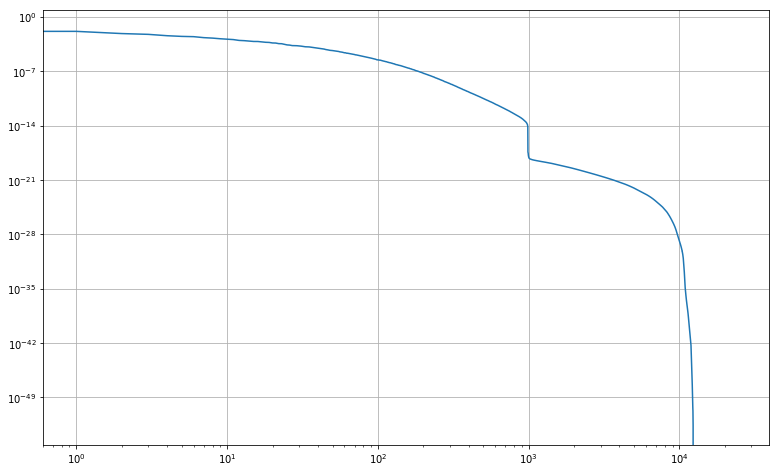
\includegraphics[width=0.8\linewidth]{figures/Covariance/Tracer_23643/cov_emp_eigenval_loglog}
    \caption{Empirical Covariance : Eigenvalues}
    \label{fig:cov:emp:eigs}
\end{figure}

So the sample covariance matrix can't be directly used for our optimisation.  

\subsection{Shrinkage Covariance}

In this section we show the results of the class of shrinkage covariance estimators. We use a simple \textbf{shrinkage} with shrinkage constant $\rho = 0.1$ and $\rho = 0.5$,  the \textbf{Ledoit-Wolf} Shrinkage and the \textbf{OAS} Shrinkage. 

\begin{table}[h]
\centering
    \begin{tabular}{|l|ccccc|}
     \hline
        & SignDet & LogDet & $\lambda_1$ & $\lambda_p$ & $\rho$ \\ \hline
        Empirical & ($-$) & $-1'399'936.28$ &  $0.0219$ & $-6.8929 \cdot 10^{-18}$ & -\\
        Shrinkage $\rho=0.1$ & ($+$) & $-351'807.64$ &  $0.0219$ &$3.3603\cdot 10^{-7}$ & $0.1$\\
        Shrinkage $\rho=0.5$ & ($+$) & $-314'035.58$ &  $0.0219$  &$1.6801 \cdot 10^{-6}$ & $0.5$\\
        Ledoit-Wolf & ($+$) & $-406'320.19$&  $0.0219$ & $3.2867\cdot 10^{-8}$ & $0.0097811$\\
        OAS & ($+$) & $-408'903.33$ & $0.0219$ & $2.9435\cdot 10^{-8}$ & $0.0087595$ \\  \hline
    \end{tabular}
    \caption{Shrinkage Comparison}
\end{table}

\begin{figure}[h!]
\centering
    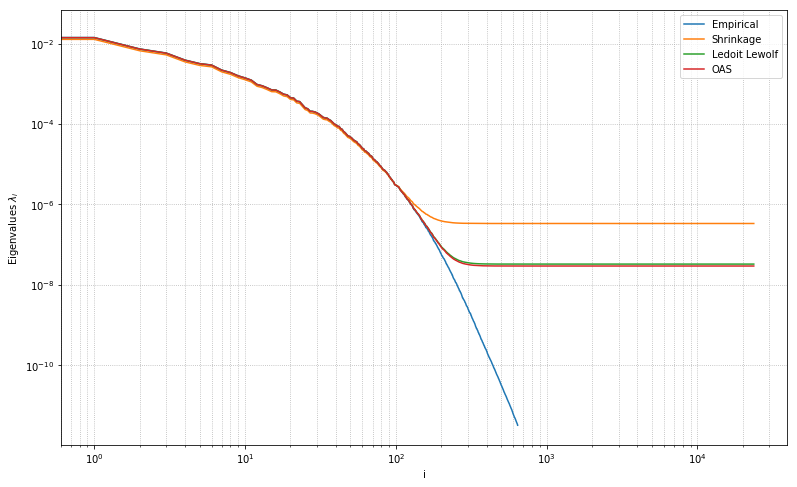
\includegraphics[width=0.8\linewidth]{figures/Covariance/Tracer_23643/cov_all_eigenval_loglog_zoom}
    \caption{Eigenvalues Covariance Comparison}
    \label{fig:cov:comparison:eigs}
\end{figure}

\todo{Comment and Compare shrinkage versions}

%\subsection{Covariance on other fields}

\subsection{Arbitrary Covariance Function}

\todo{Maybe not}





%%%%%%%%% COMPARISON %%%%%%%%

\section{Comparison Optimisation Algorithms}

We have defined the three algorithms allowing for a near-optimal placement of the sensors. In order to compare their performance and measure their limitation, we have run them on a small dataset, a subset of our main one. 
\subsection{Conditions of the Experiment}

We have defined a sphere of radius $25$m, centred close to the centre, in the middle of the propagation beam, at position $[60,35,0]$ in which are contained $3'130$ points of the mesh. By taking the intersection between those points and our selection defined in \ref{sec:preselection} , we can reduce the number of points $|S|$ to $1'295$.  The candidates are presented in figure  XX \\

\begin{figure}[h!]
\centering
    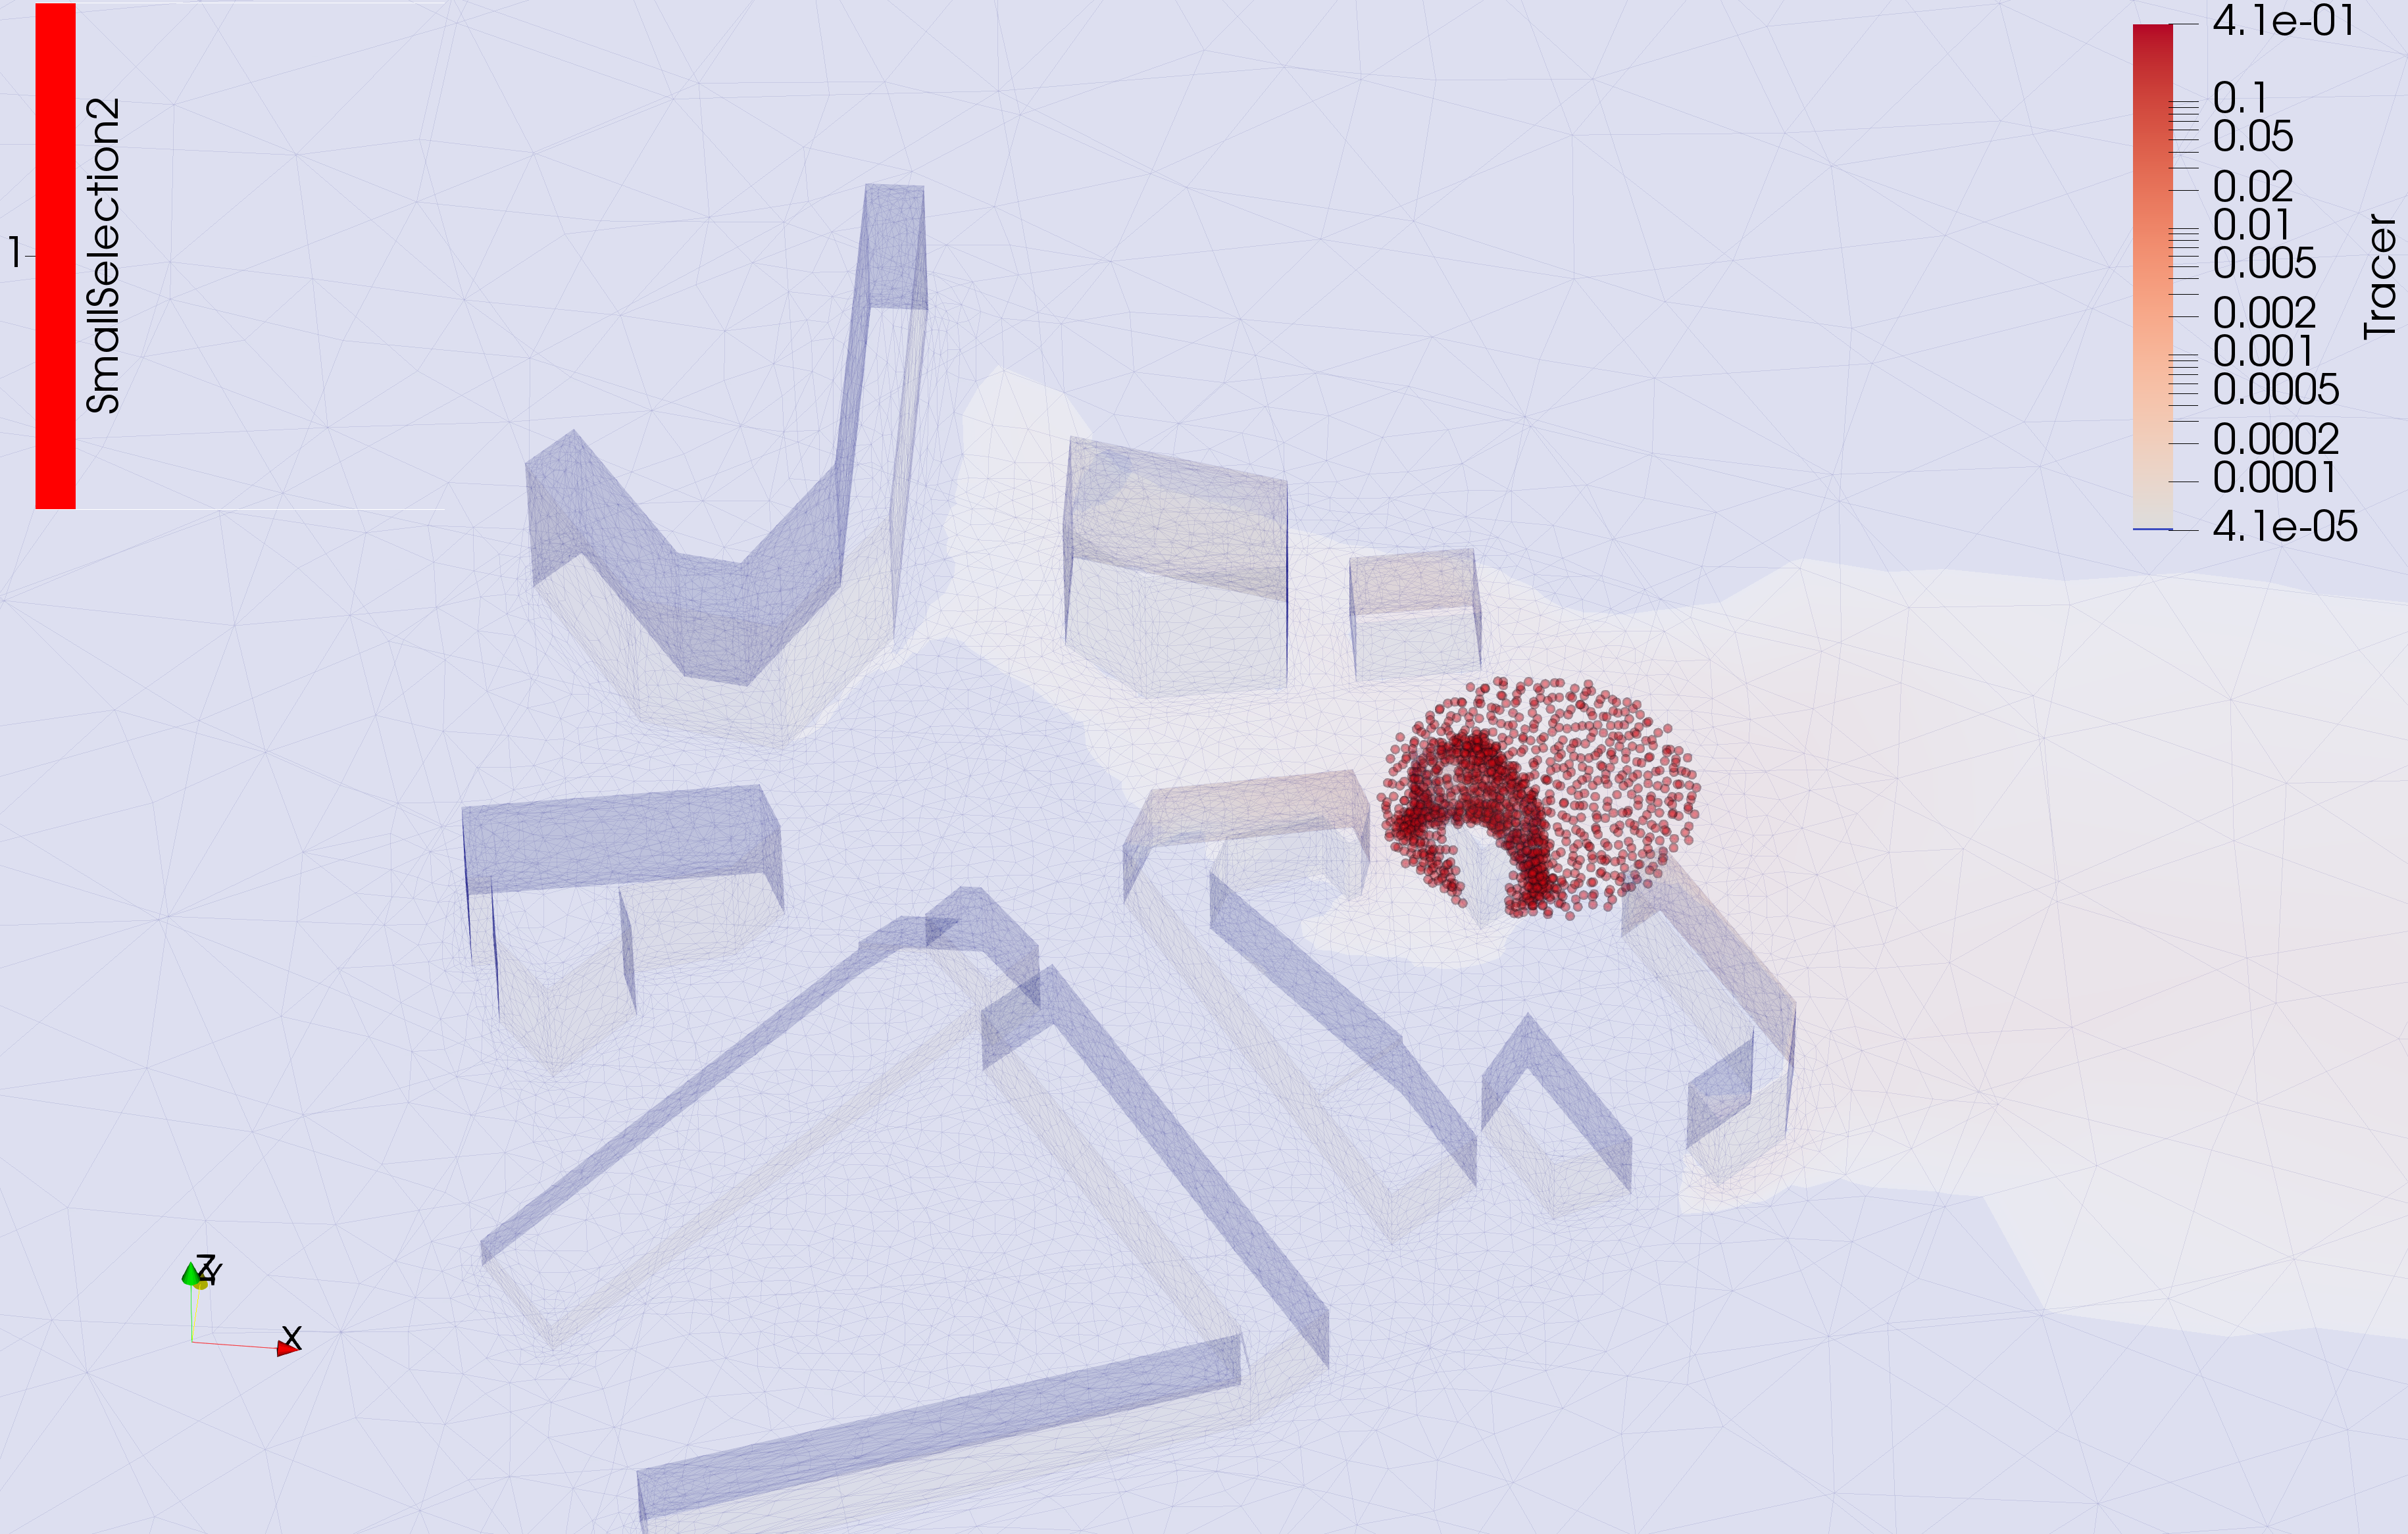
\includegraphics[width=0.8\linewidth]{figures/CompAlg/3rd/non_centered_60.35.0/candidates_screenshot}
    \caption{Small Subset Candidates}
\end{figure}

We compute the OAS covariance for this dataset and we will use in in the rest of the experience. The eigenvalues decomposition is shown for both the empirical covariance and the OAS estimate in figure \ref{fig:small_cov_eig}. \\

\begin{figure}[h!]
\centering
    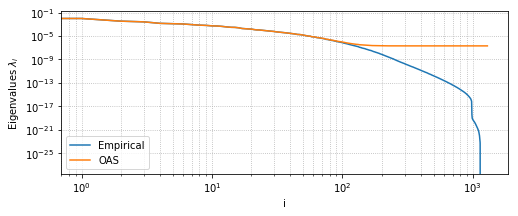
\includegraphics[width=0.7\linewidth]{figures/CompAlg/covarianceEmpOAS}
    \caption{Spectrum of Empirical and OAS covariances for small dataset}
    \label{fig:small_cov_eig}
\end{figure}

Next, we are going to optimise in this space $k=10$ points with the different algorithms and compare them based on their computation time and their distance between the datasets using the NN distance defined in \ref{equ:distNN} . 

\subsection{Greedy and Lazy Optimisation}

First, we optimise using the two first algorithms, the \textbf{greedy} and the \textbf{lazy} versions of the near-optimal sensor positioning algorithms. We will consider the output of the first algorithm as the reference for this comparison. This is because the first algorithm is the most reliable version as it covers every candidate point in its loops and relies on full GP implementation.  \\


We observe immediately that output sets given by the two methods are the same. The main difference is as expected the computation time which is much larger in the first algorithm. The Greedy Optimisation gives a result after $1043.27$s and the \textit{lazy} Optimisation gives results after $153.51 $s. The second algorithm is, for this small dataset, seven times faster than the greedy one: this is a significative difference. \\ 

The location of those points optimal points $\A^*$ is shown in green in the figure \ref{fig:opt_small} and table \ref{tab:opt_small}. We observe that the points are well spread across space and along the wind direction. As the wind is propagating the tracer concentration, it makes sense that the sensors must be placed along this direction. \\

\begin{figure}[h!]
\centering
    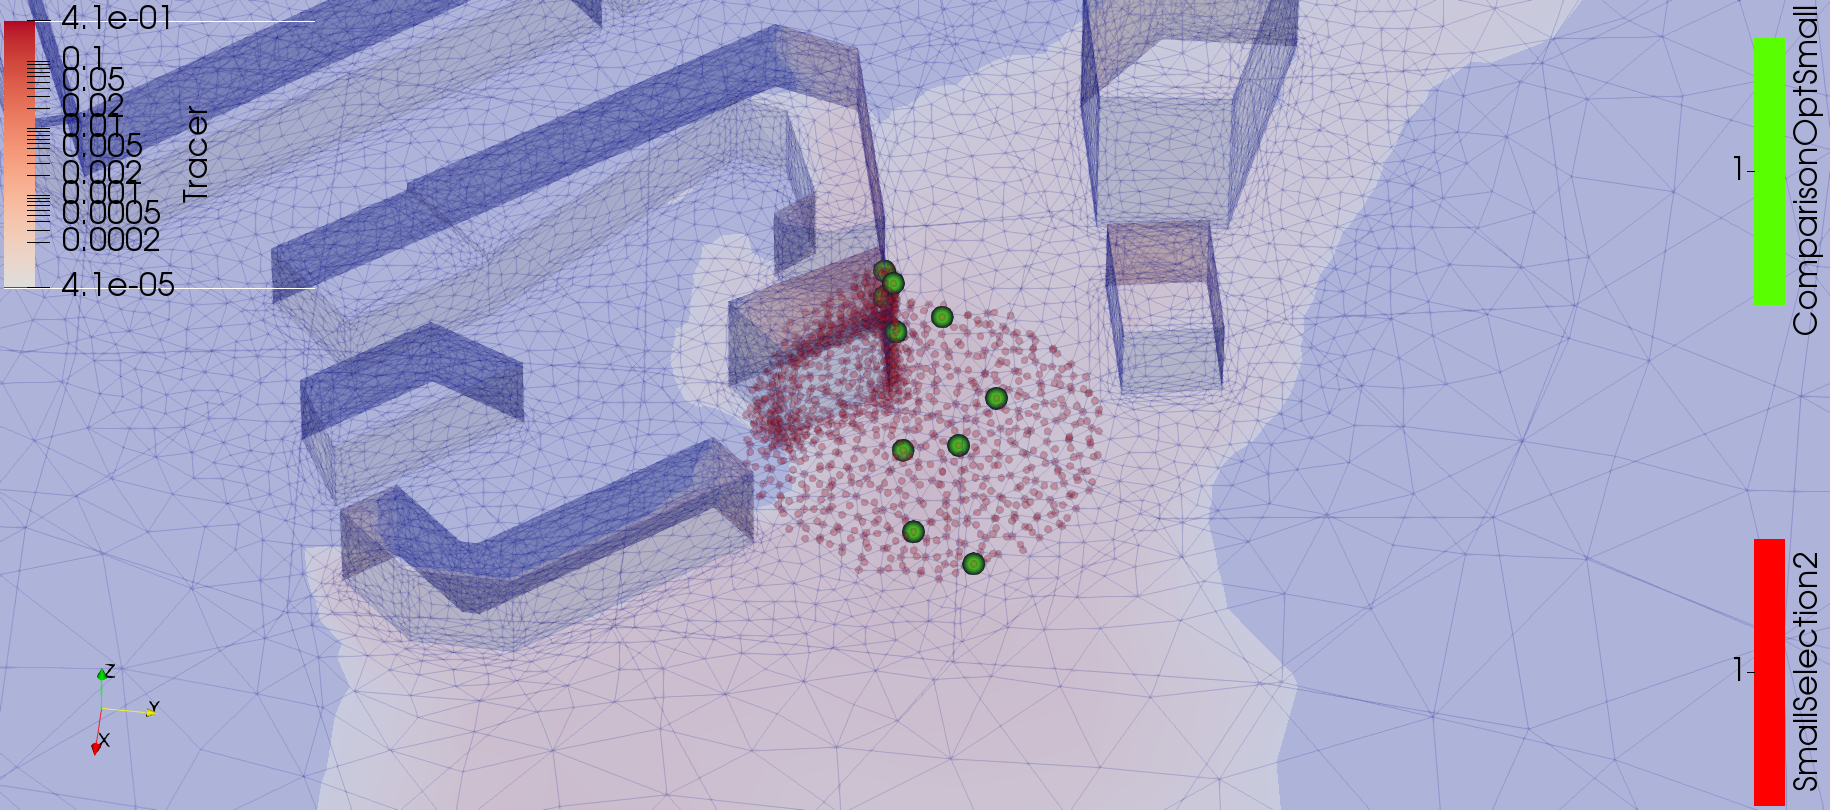
\includegraphics[width=0.8\linewidth]{figures/CompAlg/3rd/non_centered_60.35.0/optimal_screenshot}
    \caption{Optimal Points Location : Illustation}
    \label{fig:opt_small}
\end{figure}

\begin{table}[h]
\centering
\footnotesize
\begin{tabular}{|l|rrrrrrrrrr|}
\hline
$\A^*$ &  52731 &  47876 &  3078  &  19782 &  26045 &  30511 &  26754 &  81507 &  11608 &  3903  \\
\hline
X &  61.31 &  43.55 &  77.31 &  38.75 &  48.23 &  50.48 &  52.36 &  43.10 &  82.40 &  62.01 \\
Y &  40.06 &  27.62 &  35.55 &  35.26 &  29.38 &  30.04 &  44.37 &  27.52 &  44.48 &  32.39 \\
Z &   1.52 &  16.40 &   1.45 &   1.80 &  19.53 &  11.79 &   1.62 &  10.23 &   1.96 &   0.20 \\
\hline
\end{tabular}
\caption{Optimal Points Locations : Data}
\label{tab:opt_small}
\end{table}

\subsection{Local Kernels Optimisation}

The 3rd Algorithm that we are going to use is the one that is scalable to larger datasets. This scalability is dependent on the parameter $\epsilon$, the thresholding parameter of the covariance. As a consequence the number of selected covariates  $|N(y_{opt},\epsilon)| \leq d $ is fluctuating and influences greatly the speed of the algorithm. It is directly linked to the GP and the size of the covariance matrix to invert.  \\ 

This is why the threshold $\epsilon$ has to be chosen carefully. We are going to show that the speed, the NN distance and the parameter d varies according to $\epsilon$, before choosing a value that will be used for the full-scale optimisation. We compute of a range of values for $\epsilon$ all those results and show them in table \ref{tab:comp:results} and in figure \ref{fig:comp:results}. \\



\begin{table}[h!]
\centering
\scriptsize
\begin{tabular}{|l|c|c|c|c|c|c|c|c|c|c|}
  \hline
  Threshold $\epsilon$ & $10^{-10} $ &  $10^{-9}$ & $10^{-8}$ & $10^{-7}$ & $10^{-6}$ & $10^{-5}$ & $10^{-4}$ & $10^{-3}$ & $10^{-2}$ & $10^{-1}$ \\
    \hline
  Distance [m]       &    0.00 &    0.00 &    0.00 &    0.00 &   1.248 &  2.783 & 4.693 & 11.058 & 11.058 & 11.058 \\
Time [s]       & 1660.85 & 1617.92 & 1500.63 & 1151.68 &  520.36 &  60.88 &  2.44 &   1.74 &   3.25 &   2.13 \\
Average d & 1289.40 & 1288.20 & 1284.80 & 1245.60 & 1029.60 & 510.50 & 15.20 &   0.00 &   0.00 &   0.00 \\
  \hline
\end{tabular}
\caption{Local Kernel Results}
\label{tab:comp:results}
\end{table}

\begin{figure}[h]
\centering
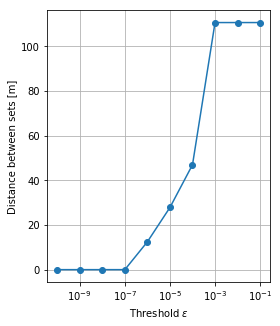
\includegraphics[height=0.33\linewidth]{figures/CompAlg/3rd/non_centered_60.35.0/comp_dist}
~
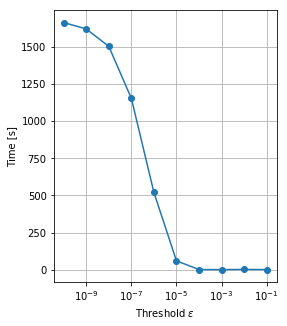
\includegraphics[height=0.33\linewidth]{figures/CompAlg/3rd/non_centered_60.35.0/comp_Time}
~
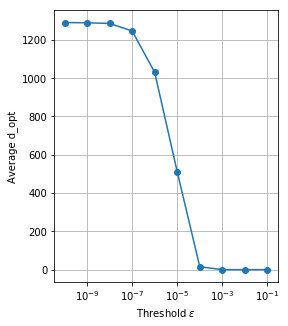
\includegraphics[height=0.33\linewidth]{figures/CompAlg/3rd/non_centered_60.35.0/comp_d_opt}
\caption{Local Kernels : Distance, Time and d, in function of $\epsilon$}
\label{fig:comp:results}
\end{figure}

We see that computation time is correlated with the average number of correlates d. For a threshold bellow $10^{-7}$, we see that the algorithm selects almost every point available and therefore we have computation times of the order of the greedy algorithm. The optimised set of points is then also the same as the greedy and lazy algorithms.\\

By increasing the threshold, we find that the computation time and the number of covariates decrease at the expense of the accuracy represented by the increase in the NN distance between this dataset and the optimal one. We observe also that for $\epsilon > 10^{-3}$, the number of covariates selected d is equal to zero which means that the algorithm updates every position at each iteration and uses for the optimisation only the values of the original covariance, without conditioning them, as the observed set is empty.  \\

Therefore we need to \textbf{fix the threshold} at around $ \epsilon_{opt} = 10^{-6}$, so that the error is still small and the computation time substantially reduced. \\ 


By moving the centre of the selection sphere, we observe that the optimal threshold is very different from one zone to the other. For example, if we place the subset in a zone where the tracer data is almost always null, we see that the threshold needs to be much smaller to get results. This is why the value we have chosen was optimised for an area where there is some data. 


\subsection{Approximated Gaussian Processes}

Alternatively, we use the approximation method developed earlier relying on the TSVD of the data, applied to algorithm 2. We proceed to the optimisation of the dataset using different values for the truncation parameter $\tau$. We then plot the computation time and the set distance to the results of the greedy algorithm in function of the truncation parameter in figure \ref{fig:small_set:tsvd}.

\begin{figure}[h]
\centering
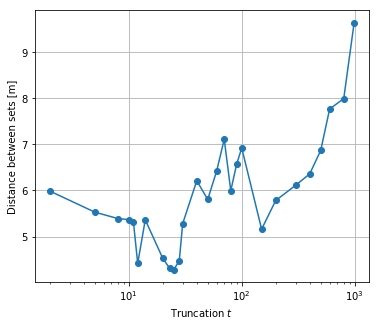
\includegraphics[height=0.33\linewidth]{figures/CompAlg/tsvd/dist_trunc}
~
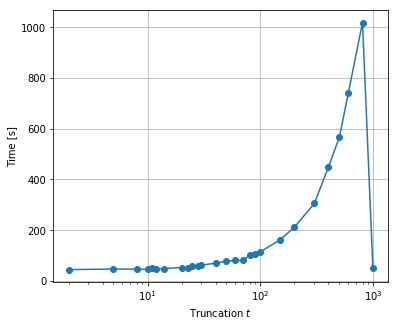
\includegraphics[height=0.33\linewidth]{figures/CompAlg/tsvd/time_trunc}
\caption{TSVD Approximation : Distance and Time in function of $\tau$}
\label{fig:small_set:tsvd}
\end{figure}

As we can see the computation time increases exponentially with $\tau$ and it is then reduced when $\tau$ gets larger than $n=988$.  For the distance between the sets and the optimal results of algorithm 1, we see that it is quite low at the beginning, is reaches a minimum at $\tau_{opt} = 25$ and it then increases this the truncation parameter. We will keep this method for trying it on the full dataset in the next section. 

%
%
%\begin{table}
%\centering
%\scriptsize 
%    \begin{tabular}{lrrrrrrrrrrrrrrrrrrrrrrrrrrr}
%\hline
% &   2   &   5   &   8   &   10  &   11  &   12  &   14  &   20  &   23  &   25  &   28  &   30  &   40  &   50  &   60  &   70  &   80  &    90  &    100 &    150 &    200 &    300 &    400 &    500 &    600 &     800 &   989 \\
%\hline
%dist & 59.87 & 55.30 & 53.91 & 53.66 & 53.15 & 44.17 & 53.63 & 45.27 & 43.13 & 42.82 & 44.74 & 52.78 & 62.10 & 58.05 & 64.22 & 71.09 & 59.93 &  65.64 &  69.20 &  51.60 &  57.82 &  61.12 &  63.61 &  68.67 &  77.67 &   79.92 & 96.42 \\
%time & 43.52 & 46.03 & 45.33 & 44.59 & 48.38 & 44.93 & 47.97 & 51.90 & 50.48 & 56.97 & 56.55 & 61.21 & 69.06 & 77.49 & 79.66 & 80.56 & 99.81 & 105.75 & 114.13 & 161.96 & 211.30 & 305.01 & 448.92 & 567.17 & 741.89 & 1018.80 & 49.40 \\
%\hline
%\end{tabular}
%\end{table}


\subsection{Arbitrary Covariance}

Alternatively, we define the covariance using an \textit{isotropic} and \textit{stationary} kernel function with arbitrary parameters. We chose for this experiment the 5/2 Matérn kernel. Unrelated to the data !!

\todo{Add in literature review // Implementation the Kernels definitions}







%\todo{Add section on the abritrary kernels results}




%%%%%%%%% OPTIMISATION %%%%%%%%

\section{Optimisation Results}

After the analysis of different algorithm results on a small sample dataset, we are now going to use the most scalable algorithms with the appropriate parameters on the full dataset. The set of points used is the preselected dataset containing $23'643$ locations. \\

In this section, we will present the results of two optimisations, compare them in term of computation speed and proximity. 

\subsection{Local Kernel Algorithm}

We first use the Local Kernel Algorithm \ref{alg:local}. The covariance between the points is computed using the OAS estimator. \\


For this experiment we used the previously defined value of threshold : $\epsilon = 10^{-6}$. Such that the number of points highly correlated to the last positioned sensor is $|N(y_{opt},\epsilon)| \leq d $. \\ 

The algorithm computes the following results in $23797.2$ seconds or $6.61$ hours. \\

We are computing for each iteration the size of this set. This number is directly linked to the size of the covariance matrix being inverted in the GPs. As we are placing 10 sensors, we have 10 values of this quantity that is computed at each iteration of the main loop. Results can be found in table \ref{tab:full:d_opt}. The average value is $4'374.7$. This shows that indeed the optimisation problem is solved in a reduced time as it doesn't use all the $23'643$ locations of our dataset, but $18.50$\% of it.   \\

\begin{table}[h]
    \centering
    \begin{tabular}{|l|cccccccccc|}
    \hline
    Sensor & 1 & 2 & 3 & 4 & 5 & 6 & 7 & 8 & 9 & 10 \\     \hline
        $|N(y_{opt},\epsilon)|$ & 4338 & 4938 & 5066 & 5362 & 4239 & 4164 & 3377 & 4632 & 3511 & 4120 \\     \hline

    \end{tabular}
    \caption{Number of highly correlated points at each iteration}
    \label{tab:full:d_opt}
\end{table}


We visualise the position of the optimal set of sensor points $\A^*$ at different scales in the figures \ref{fig:full_set:position:all}, \ref{fig:full_set:position:top} and \ref{fig:full_set:position:zoom}. The coordinates of the points are expressed in the table \ref{tab:full:data}. \\


\begin{table}[h]
\centering
\footnotesize
\begin{tabular}{|l|rrrrrrrrrr|}
\hline
$\A^*$ &  56588 &  52731 &  73959 &  43278 &  3078  &  19782 &  56257 &  55640 &  10357 &  54786 \\ \hline
X &  41.61 &  61.31 &  30.32 &  22.79 &  77.31 &  38.75 &  91.19 &  50.10 &  62.13 &   1.62 \\
Y &  27.21 &  40.06 &  26.06 &  25.81 &  35.55 &  35.26 &  35.16 &  29.00 &  45.23 &  19.99 \\
Z &  16.73 &   1.52 &  11.19 &  11.79 &   1.45 &   1.80 &   1.82 &  16.41 &   1.64 &  13.81 \\
\hline
\end{tabular}
\caption{Optimal Points Locations : Data}
\label{tab:full:data}
\end{table}



\begin{figure}[h!]
\centering
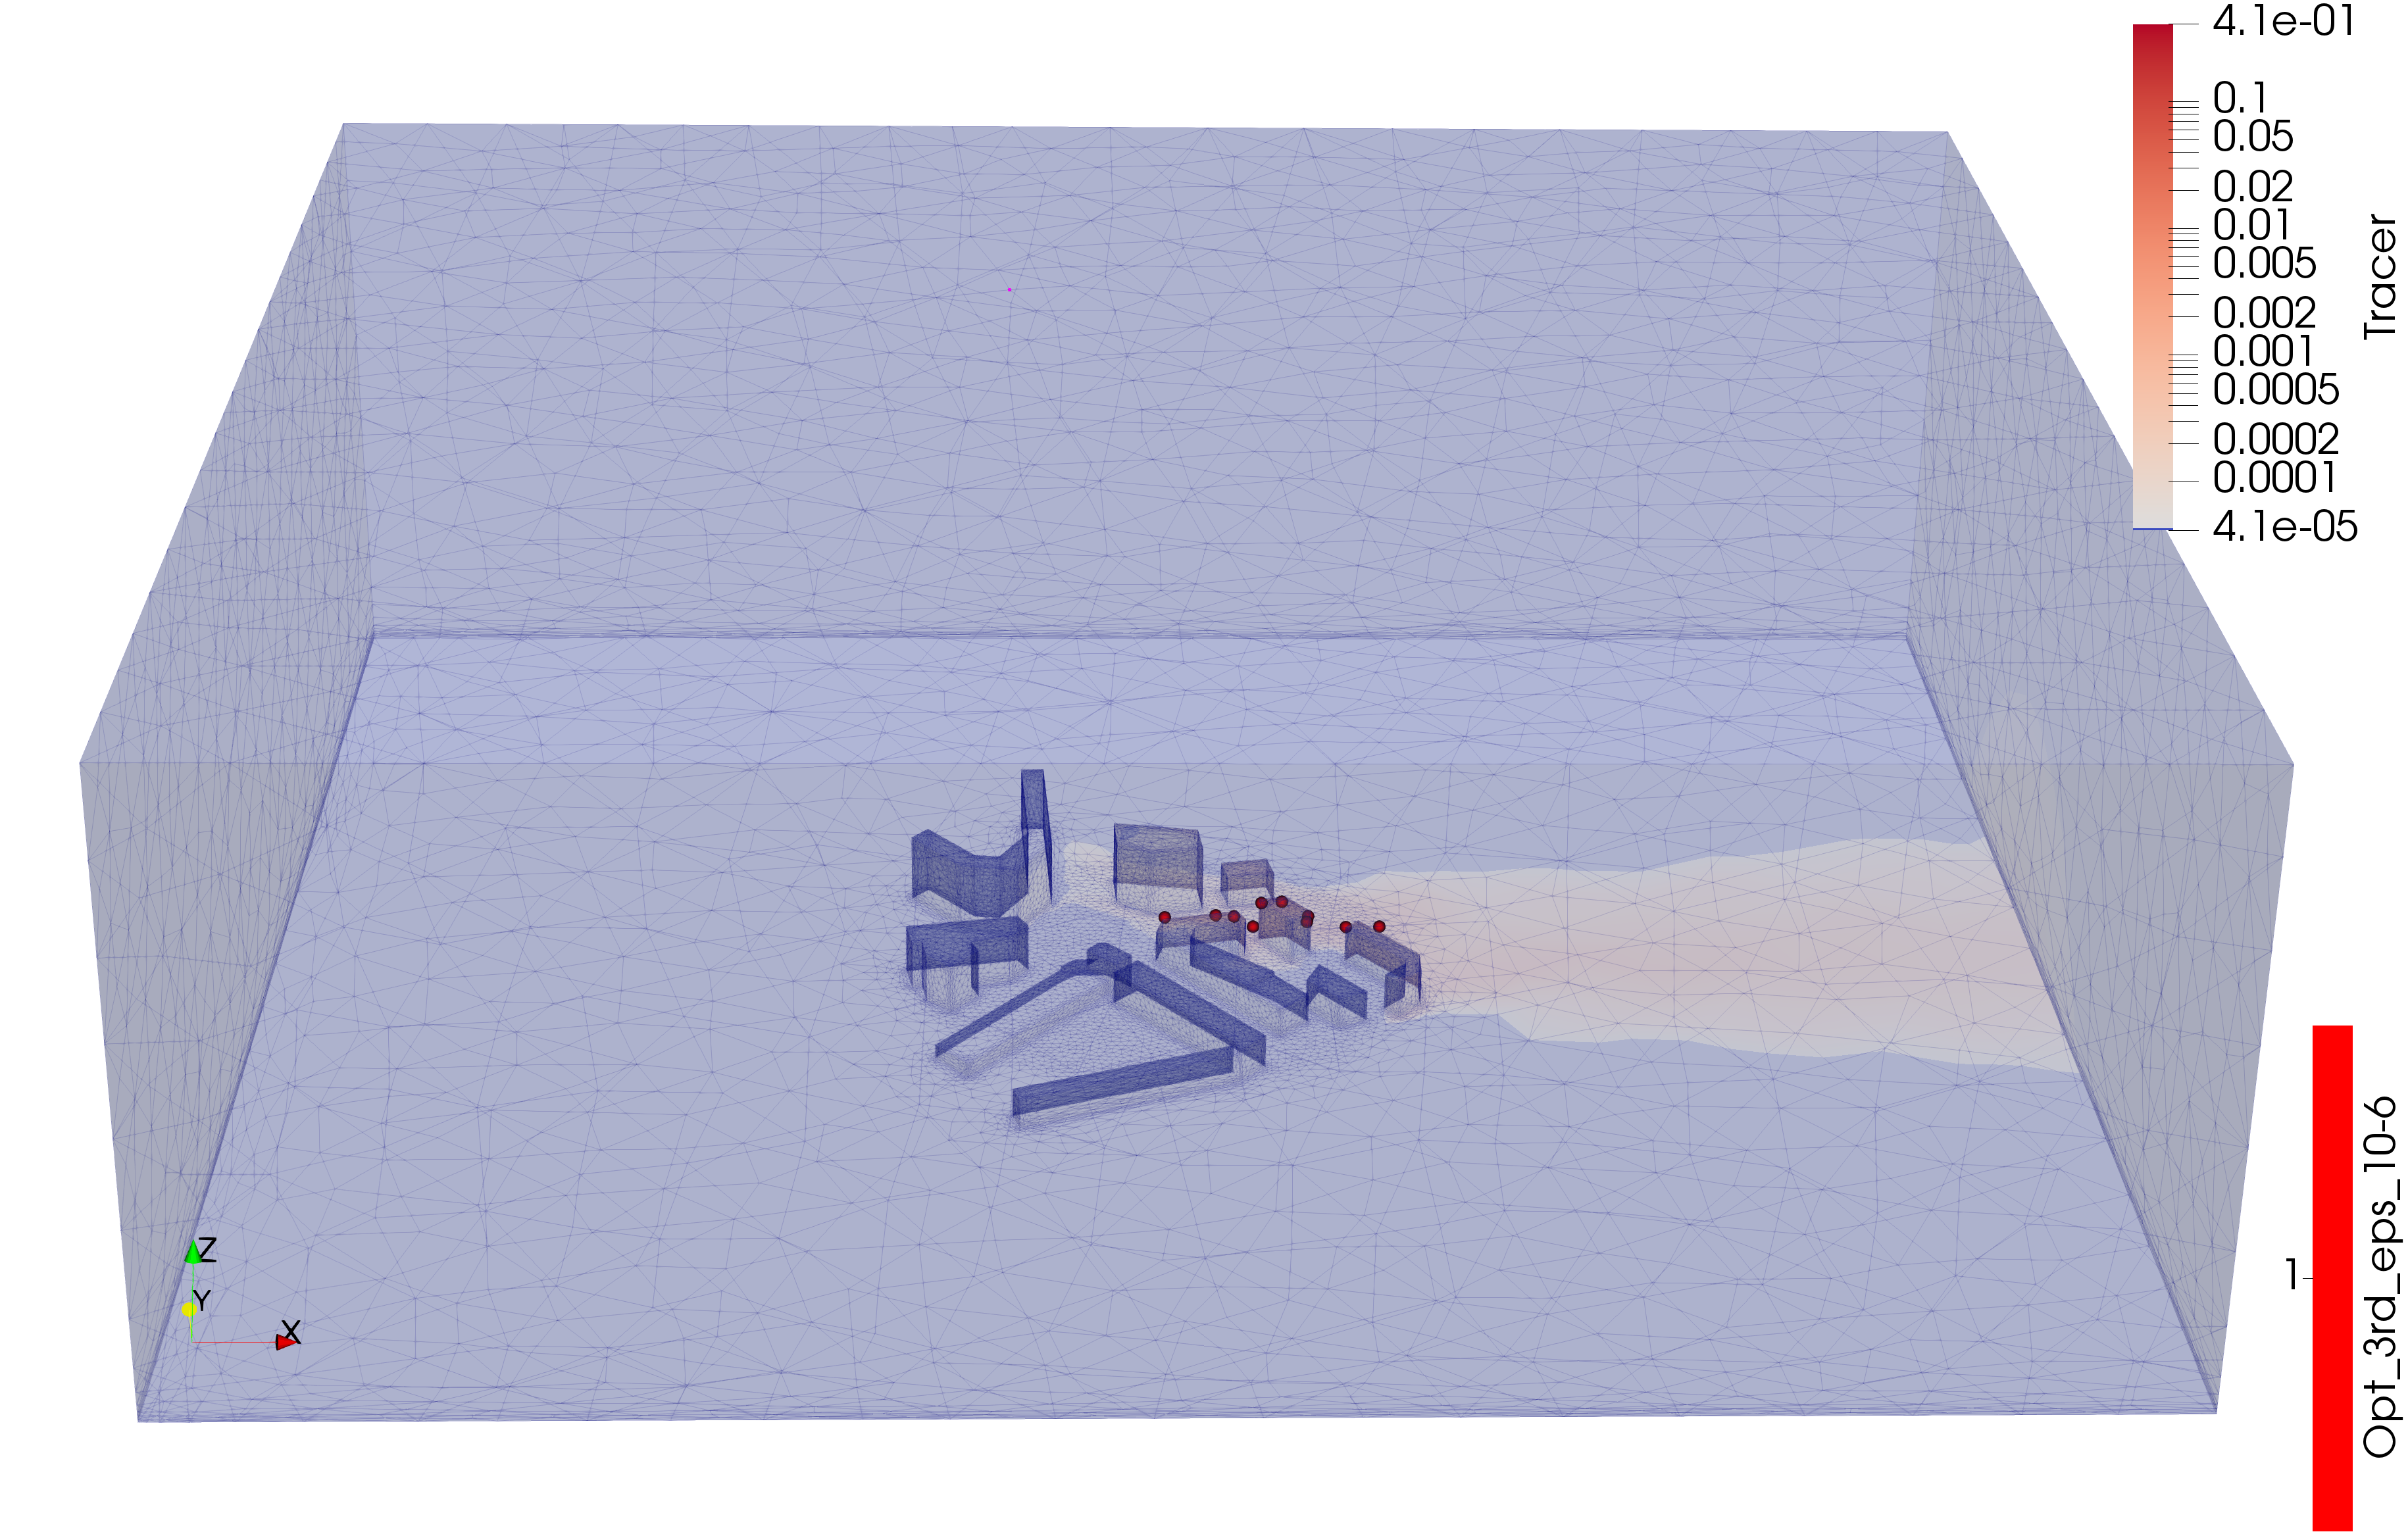
\includegraphics[width=0.7\linewidth]{figures/MainOptimResults/alg3opteps10-6_sideall_screenshot}
\caption{Position of the Optimal Set : Main View}
\label{fig:full_set:position:all}
\end{figure}



\begin{figure}[h!]
\centering
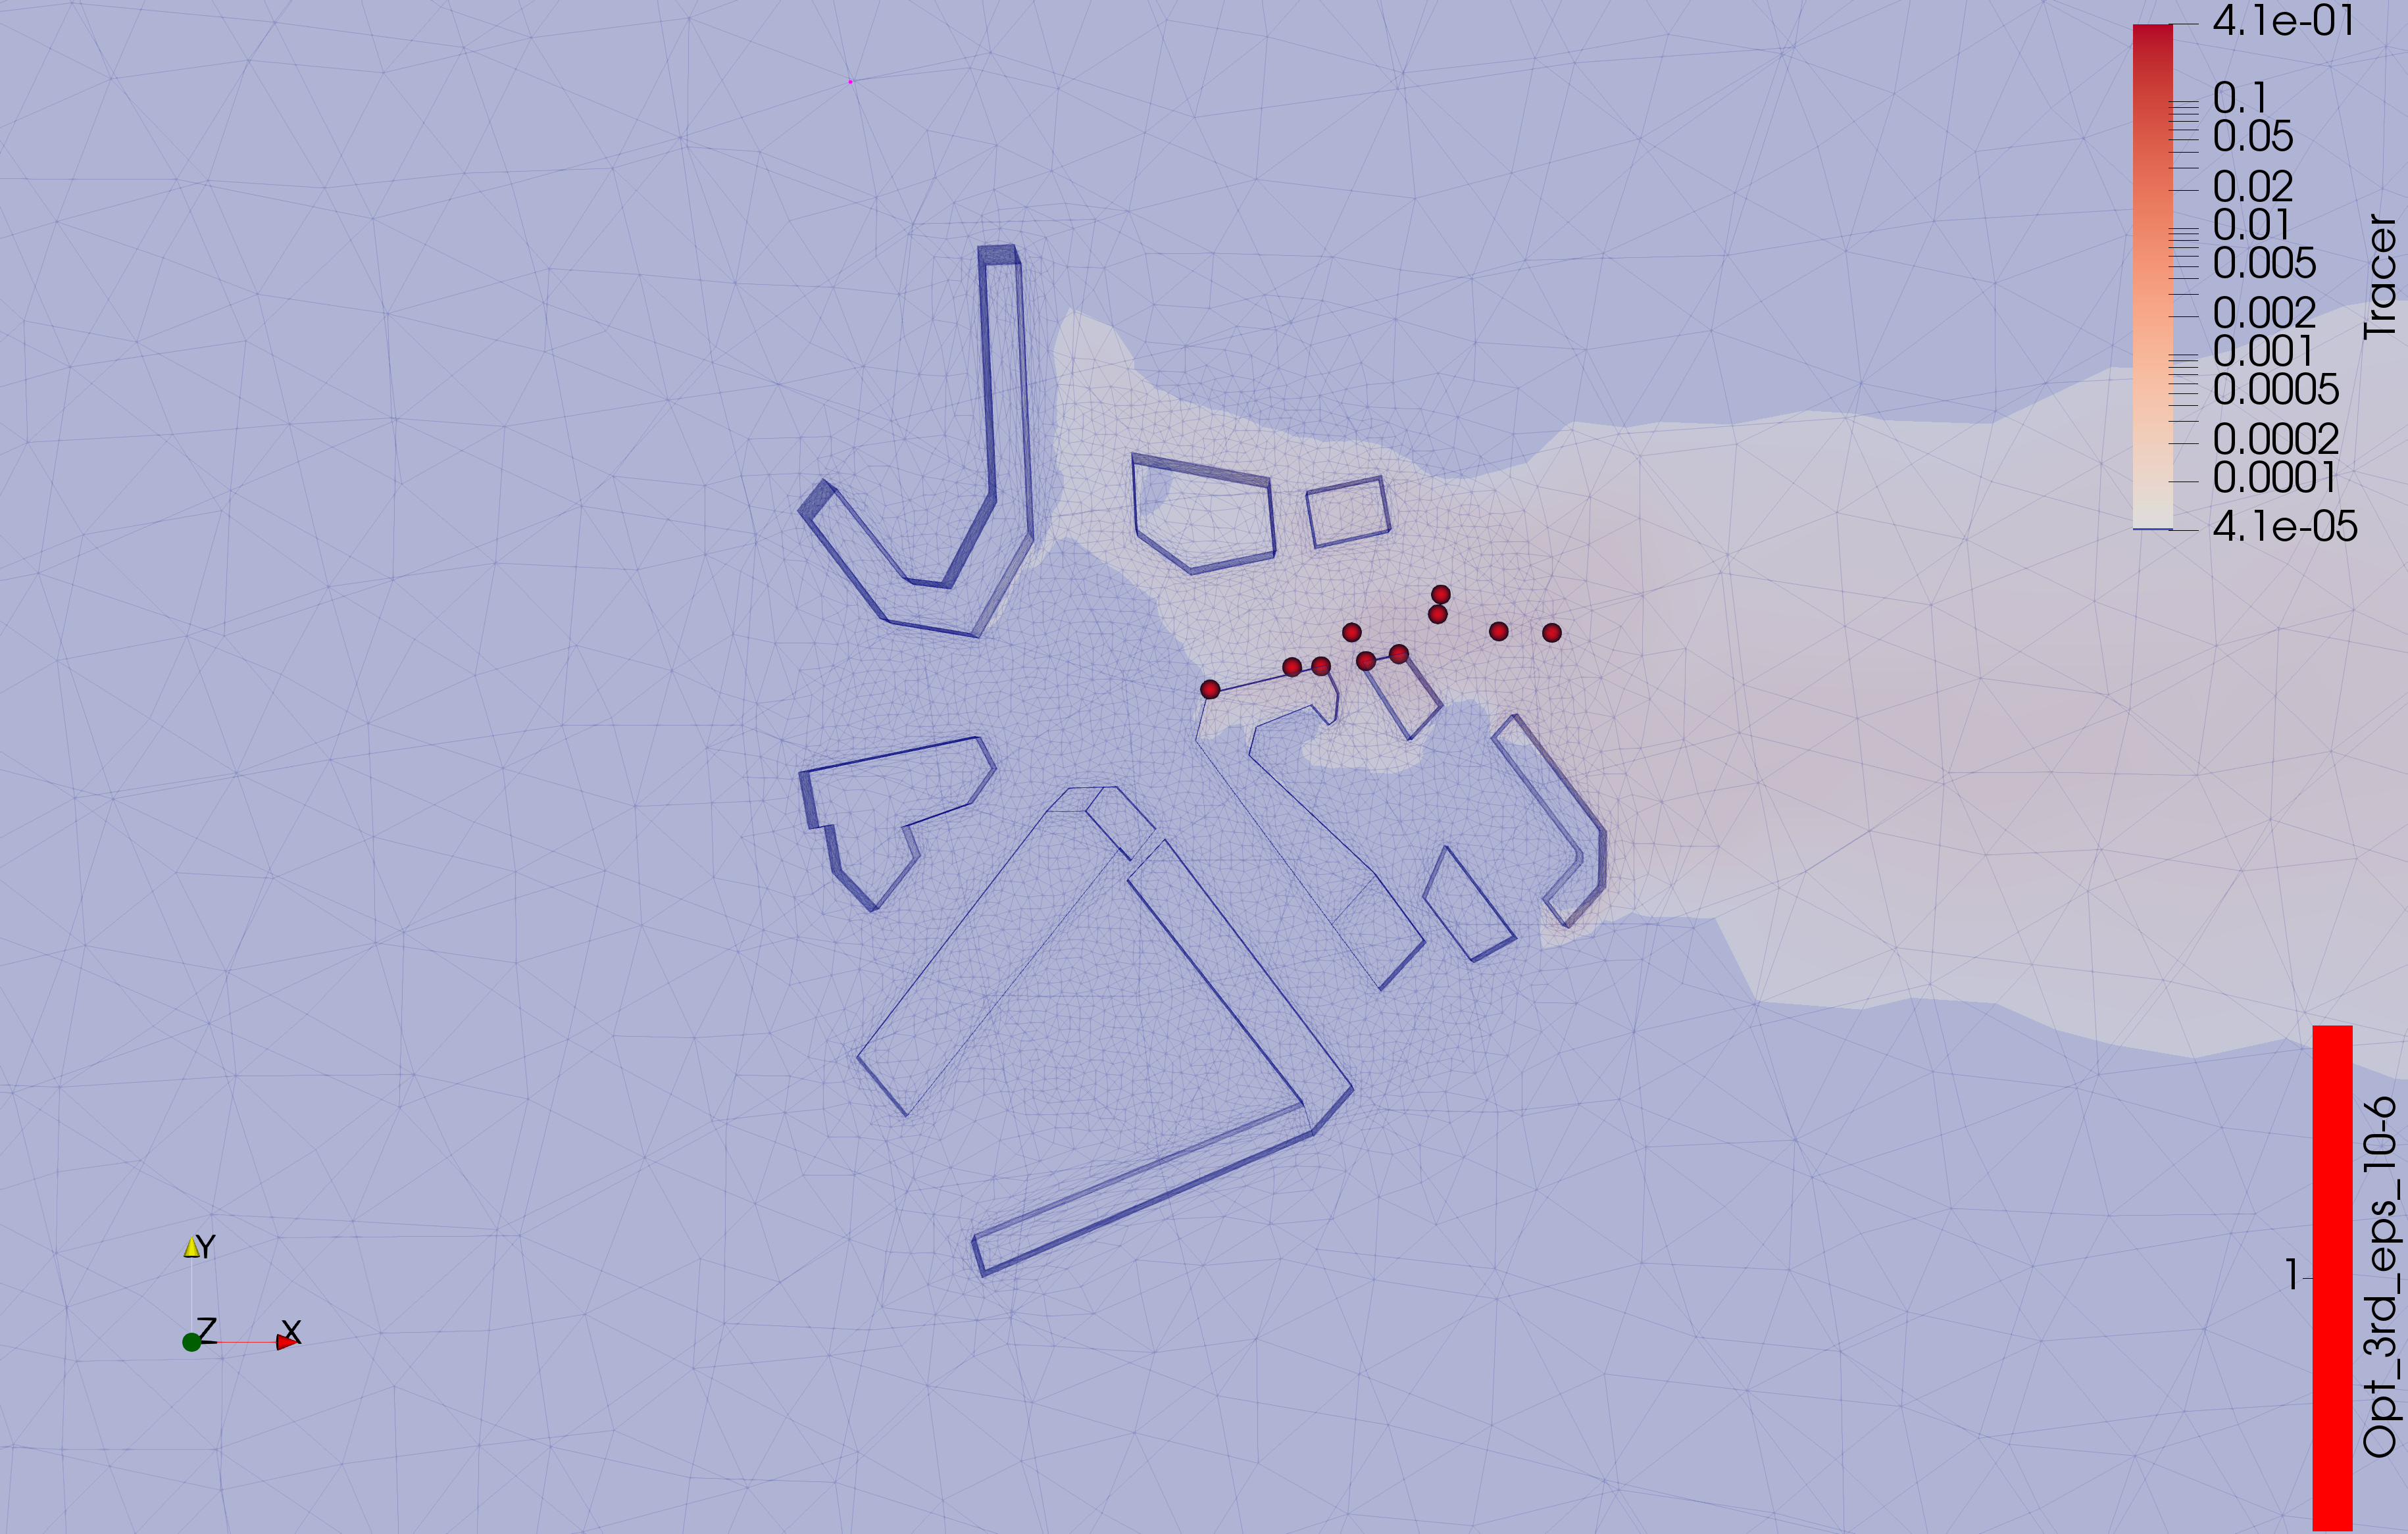
\includegraphics[width=0.7\linewidth]{figures/MainOptimResults/alg3opteps10-6_top_screenshot}
\caption{Position of the Optimal Set : Top View}
\label{fig:full_set:position:top}
\end{figure}

\begin{figure}[h!]
\centering
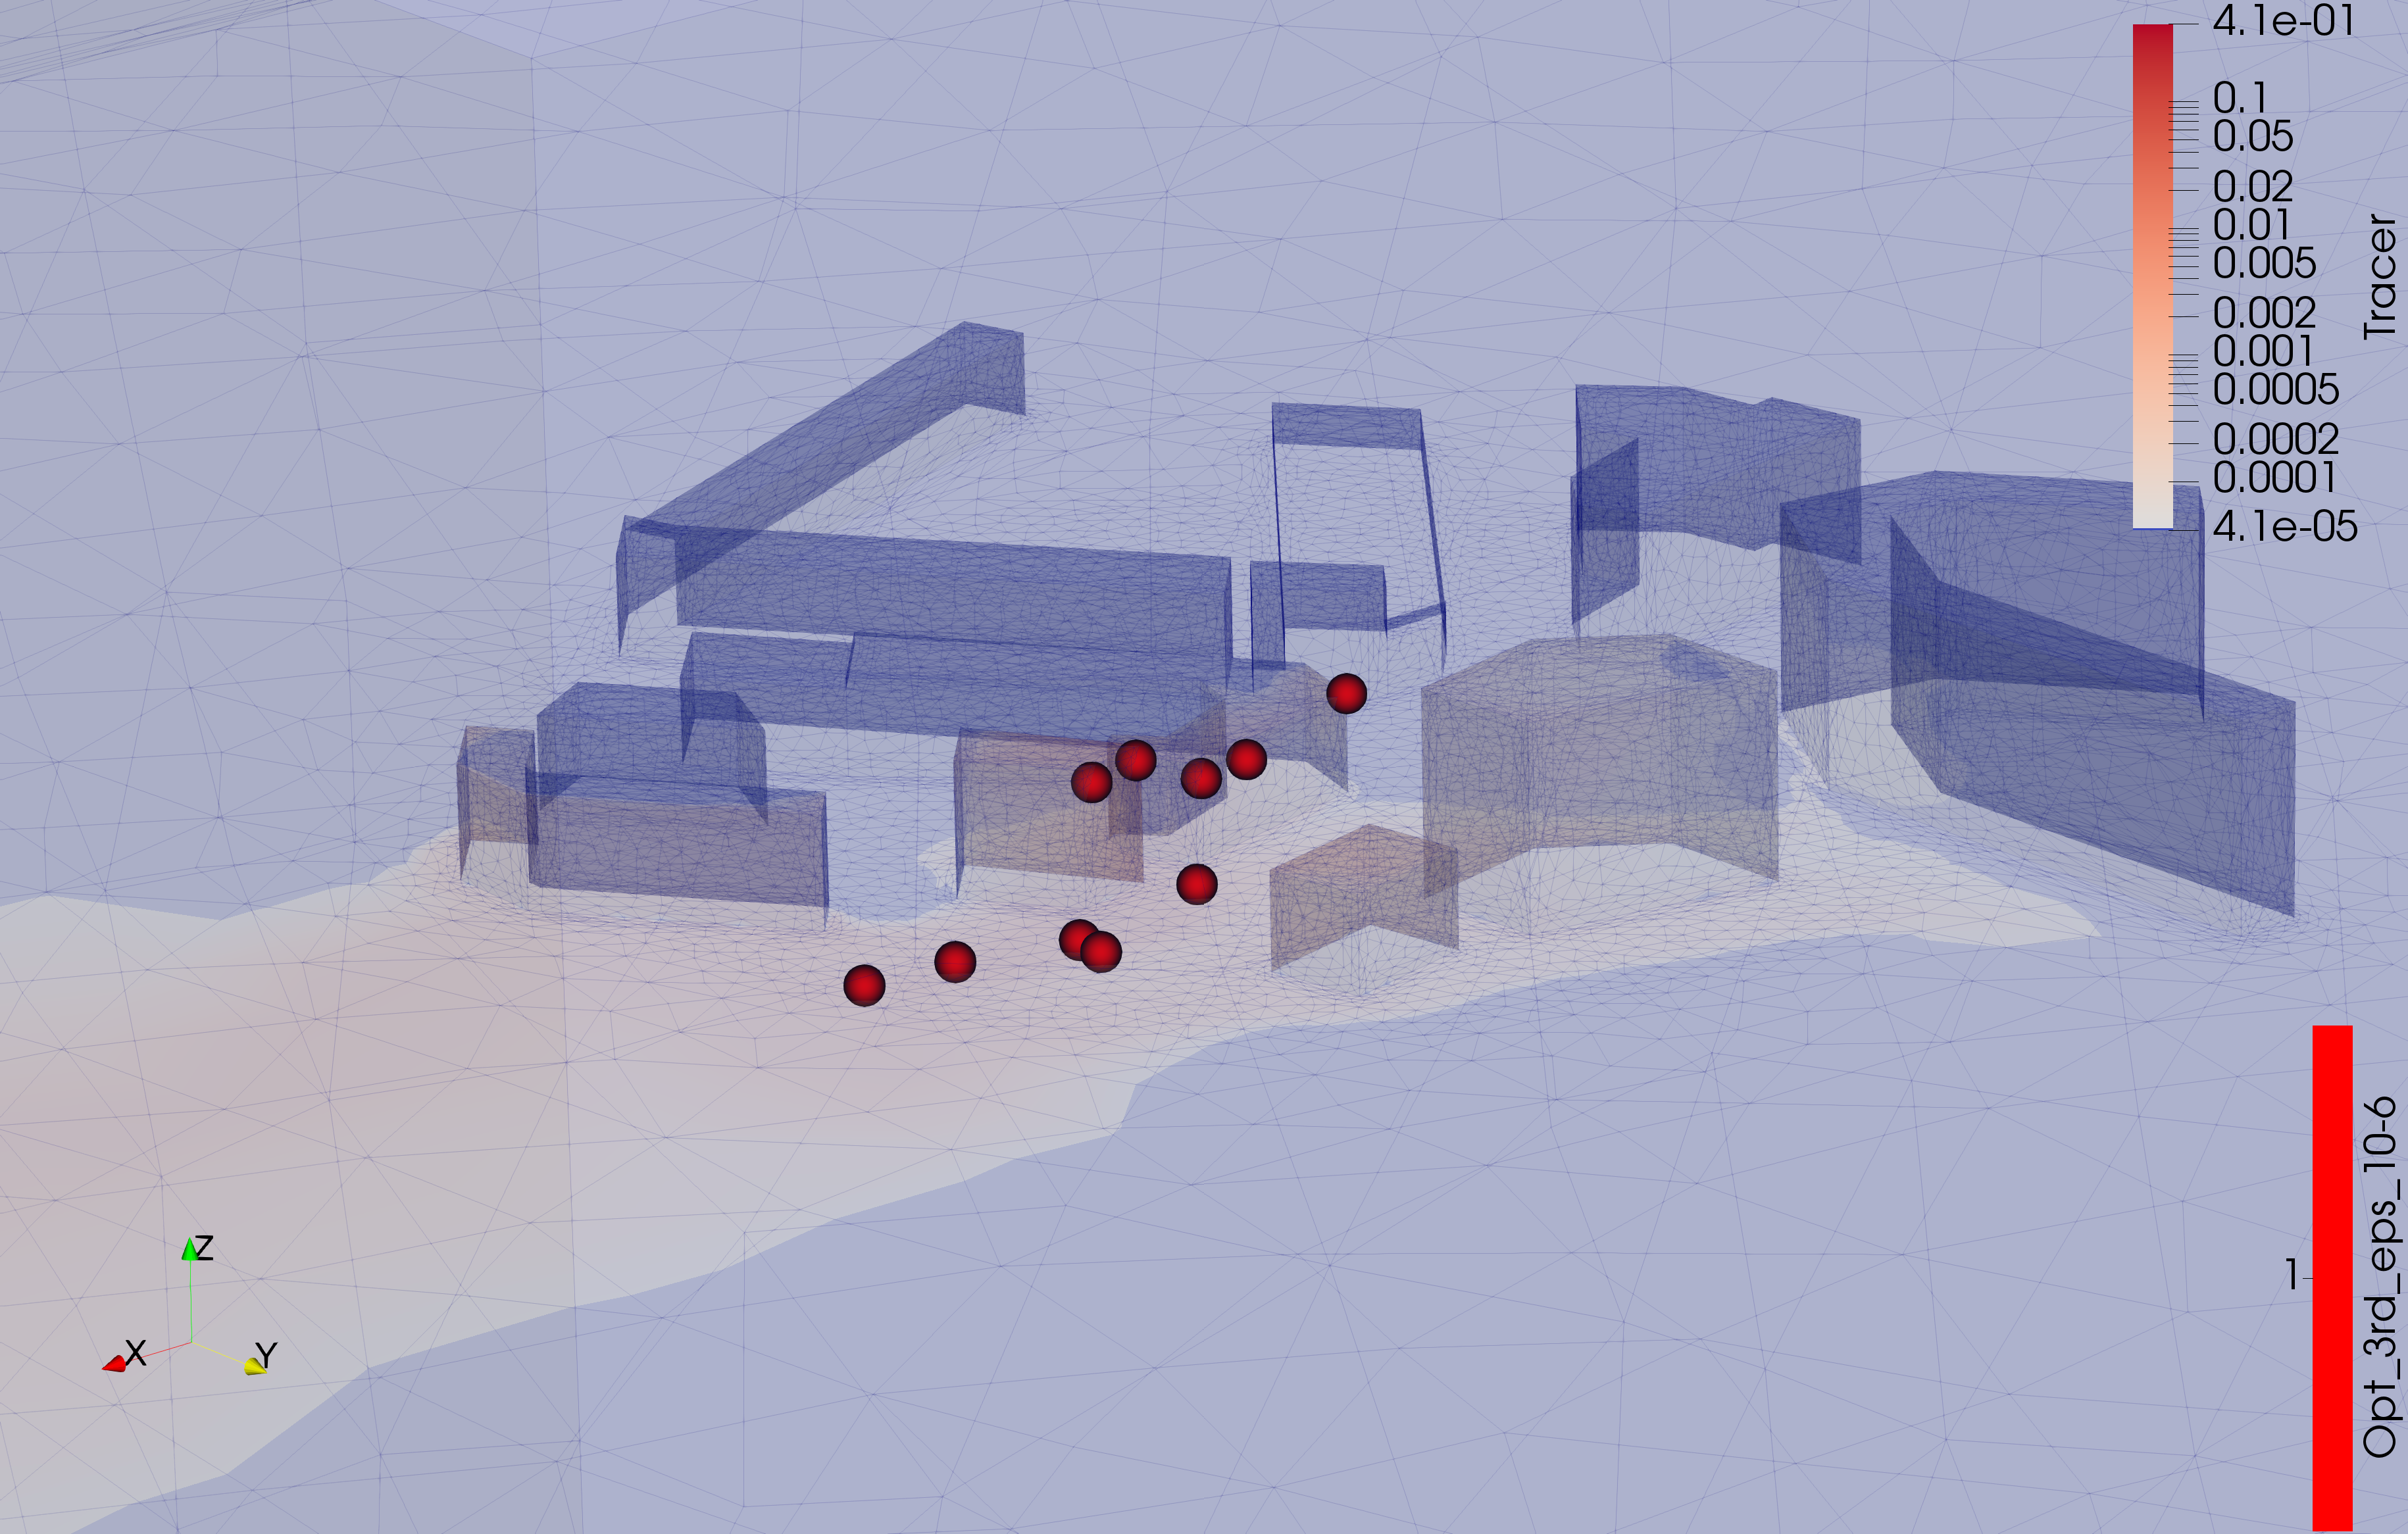
\includegraphics[width=0.7\linewidth]{figures/MainOptimResults/alg3opteps10-6_zoom_screenshot}
\caption{Position of the Optimal Set : Close View}
\label{fig:full_set:position:zoom}
\end{figure}


\paragraph{Description}

The location of our optimal set of points is split between points situated on the buildings (5 points) and around the ground level (5 points). They are situated in the middle of the tracer concentration beam and are close to the centre of the domain where the mesh density is maximal. \\ 

The points are roughly aligned in the wind direction, which seems to be a good thing because we have a propagation originating at the centre and with wind in the east direction. 


\subsection{Lazy Algorithm with TSVD}

We apply on the same dataset the 2nd Algorithm with the approximated GP that we defined earlier. We use the truncation parameter $\tau_{opt} = 25$. The results we obtain are displayed in table \ref{tab:tsvd:data}
 and figures \ref{fig:full_set_tsvd:position:top} and \ref{fig:full_set_tsvd:position:zoom} along with the previous optimal results. 
 
 \paragraph{Description}

Here again the location of our optimal set of points is split between points situated on the buildings (3 points) and around the ground level (7 points). The locations are more spread than the other set of points. Two locations are at the border the the pre-selected dataset. The distance between this set and the previous one is of : $13.84$m which is quite important.  \\ 



\begin{table}[h]
\centering
\footnotesize
\begin{tabular}{|l|rrrrrrrrrr|}
\hline
$\A^*$ &  38726 &  14276 &  91348 &  5338  &  40994 &  29626 &  65851 &  65734 &  851   &  2293  \\
\hline
X & -50.50 &  35.63 &  43.05 & 137.58 &  80.34 &  27.79 &  49.54 &  54.59 &  77.54 &  62.03 \\
Y &  48.85 &  58.69 &  27.51 &  55.78 &  76.20 &  26.24 &  28.88 &  25.42 &  34.82 &  41.92 \\
Z &  14.84 &   0.20 &   7.76 &   0.20 &   0.20 &  12.06 &  17.65 &   3.80 &   0.20 &   0.20 \\
\hline
\end{tabular}
\caption{Optimal Points Locations TSVD : Data}
\label{tab:tsvd:data}
\end{table}


\begin{figure}[h!]
\centering
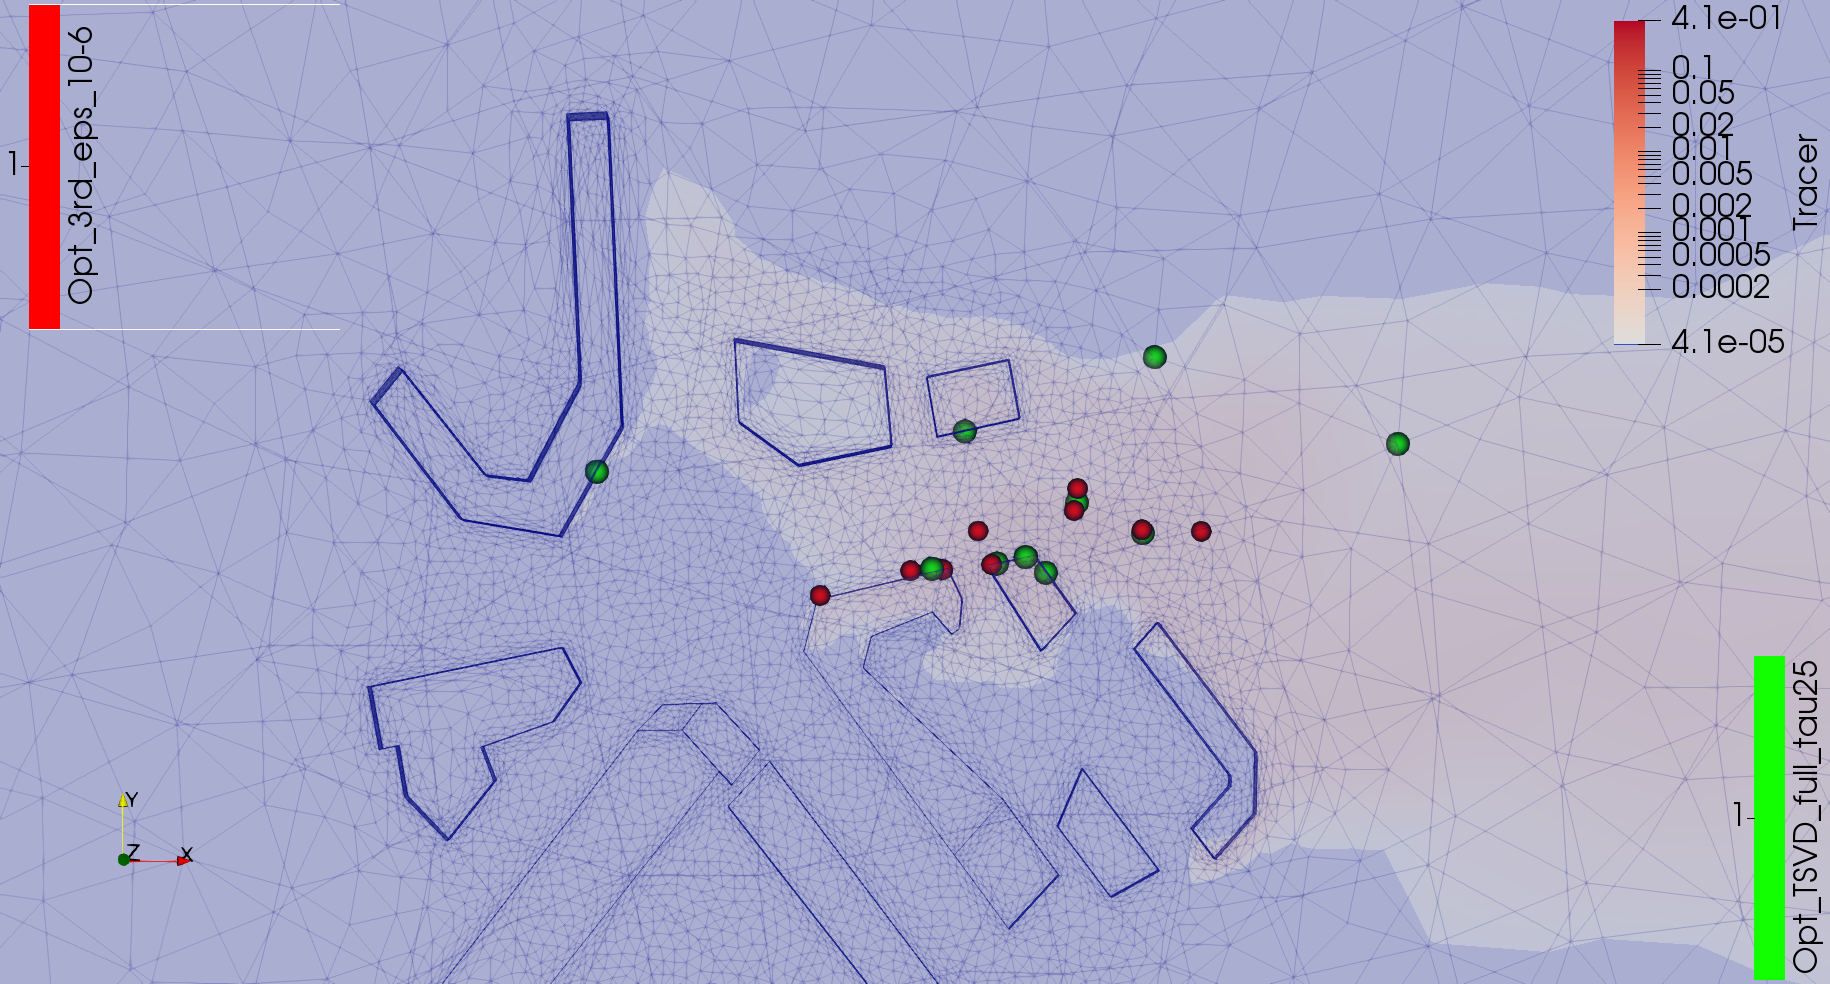
\includegraphics[width=0.7\linewidth]{figures/MainOptimTSVD/tsvd+3rd_position_top}
\caption{Position of the Optimal Set : Main View - $\tau = 25$}
\label{fig:full_set_tsvd:position:top}
\end{figure}

\begin{figure}[h!]
\centering
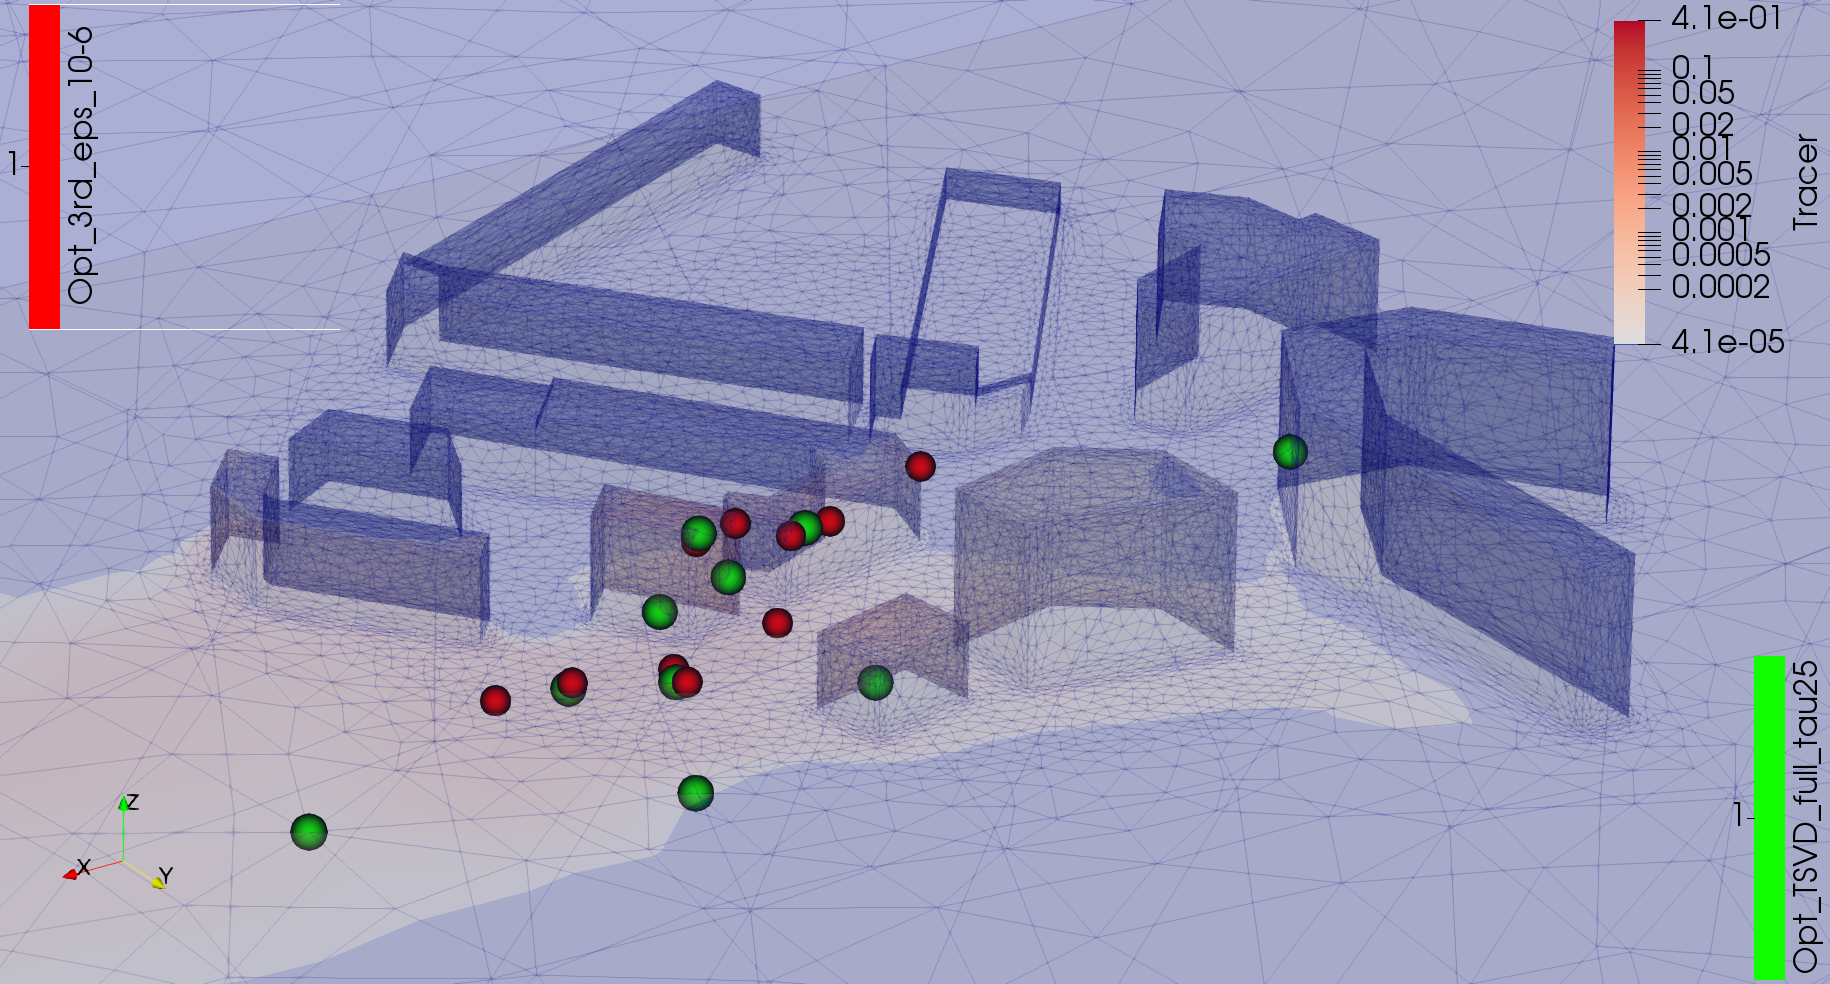
\includegraphics[width=0.7\linewidth]{figures/MainOptimTSVD/tsvd+3rd_position_side}
\caption{Position of the Optimal Set : Main View $\tau = 25$}
\label{fig:full_set_tsvd:position:zoom}
\end{figure}







%%%%%%%%% OPTIMISATION %%%%%%%%

\section{Validation with VarDA}

\todo{Add Validation Results}
